\documentclass[a4paper,11pt,notitlepage,fullpage]{article}
%\documentclass{report}

\usepackage{fullpage}
\usepackage[utf8]{inputenc}
%\usepackage[ngerman]{babel}
\usepackage[english]{babel}
\usepackage{amsmath}
\usepackage{amssymb}
\usepackage{latexsym}
\usepackage{mathtools}
\usepackage{listings}
\usepackage{algorithm}
\usepackage{algpseudocode}
\usepackage{graphicx}
\usepackage{booktabs}
\usepackage{hhline}
\usepackage{amsthm}
\usepackage{cite}
\usepackage{wrapfig}
\usepackage{hyperref}
\usepackage{titling}
\usepackage{color}

\setlength{\droptitle}{-60pt}


\begin{document}
\author{Florian Bogner}
\title{Differential Geometry - Exercise 9}
\maketitle


\begin{enumerate}
\item Let $(U_i, \phi_i)_{i\in I}$ be an enumeration of the smooth structure of M and similarly $(V_j, \psi_j)_{j\in J}$ be an enumeration of the smooth structure of N. Lots of properties held by components are also true for the products:
\begin{itemize}
\item $(U_i\times V_j)_{(i,j)\in I\times J}$ is a covering of $M \times N$ as are the components.
\item $\phi_i \times \psi_j: M\times N \to R^m \times R^n: (p, q) \mapsto \phi_i(p) \times \psi_j(q)$ is a homeomorphism for every $i \in I, j \in J$ as are the components.
\item The transition maps $(\phi_{i_1} \times \psi_{j_1}) \circ (\phi_{i_2} \times \psi_{j_2})^{-1} = (\phi_{i_1} \circ \phi^{-1}_{i_2}) \times (\psi_{j_1} \circ \psi^{-1}_{j_2})$ are diffeomorphisms as the component maps are diffeomorphisms.
\end{itemize}
Therefore $(U_i\times V_j, \phi_i \times \psi_j)_{(i,j)\in I\times J}$ is a smooth Atlas on $M\times N$. It has a unique maximal atlas as the lecture notes tell us on p.94. This is the desired natural smooth structure. \qed


\item Let 
\begin{equation*}
U_1 \subset \mathbb RP^2 = \left\{\left[x,y,z\right]_\sim \centering|~ x, y, z \in \mathbb R, z \neq 0 \right\}
\end{equation*}
and
\begin{align*}
\phi_1 :  U_1 &\to \mathbb R^2 \\
\left[x,y,z\right]_\sim &\mapsto (\frac{x}{z}, \frac{y}{z})
\end{align*}
We have the inverse as
\begin{align*}
\phi_1^{-1} : \mathbb R^2 &\to U_1 \\
(x,y) &\mapsto \left[x,y,1\right]_\sim
\end{align*}
Note that these definitions do not depend on the representation $(x,y,z)$ of $\left[x,y,z\right]_\sim$.
\begin{equation*}
\phi_1(\left[x,y,z\right]_\sim) = \phi_1(\left[\lambda x,\lambda y,\lambda z\right]_\sim) = (\frac{\lambda x}{\lambda z}, \frac{\lambda y}{\lambda z}) = (\frac{x}{z}, \frac{y}{z})
\end{equation*}
Therefore and because $z \neq 0$ they are well defined. Both $\phi_1$ and $\phi_1^{-1}$ are obviously continuous, thus $\phi_1$ is indeed a homeomorphism. 

We define $U_2, U_3$ and $\phi_2, \phi_3$ analogously swapping the roles of $z$ with $x$ and $y$ respectively. Since for $\left[x,y,z\right]_\sim \in \mathbb RP^2$ we have one of $x, y, z$ not equal to $0$, thus it is in one of $U_i$. Therefore we have an Atlas.

Finally, are the transition maps smooth? Lets consider 
\begin{equation*}
U_2 \cap U_3 = \left\{\left[x,y,z\right]_\sim \centering|~ x, y, z \in \mathbb R, x \neq 0, y \neq 0 \right\}
\end{equation*}
Then we have the transition map
\begin{align*}
\phi_3 \circ \phi_2^{-1} :  \mathbb R^2 &\to \mathbb R^2 \\
(y, z) &\mapsto \phi_3(\left[1,y,z\right]_\sim) = (\frac{1}{y}, \frac{z}{y})
\end{align*}
This is obviously smooth for $y \neq 0$. Its inverse is smooth for $x \neq 0$. This also holds for the other two transition maps analogously. Therefore we have a \emph{smooth} Atlas. \qed

\item The smooth structure generated by $id$ equals the set of all diffeomorphisms on open subsets of $\mathbb R$. However, $\phi$ is not a diffeomorphism, as its inverse is not differentiable at 0. Thus the smooth structure generated by $\phi$, which of course contains $\phi$ cannot be equal to the one generated by $id$.

$F: p \mapsto p^{\frac{1}{3}}$ is a diffeomorphism from the smooth structure of $id$ to the smooth structure of $\phi$ as
\begin{align*}
\phi \circ F \circ id^{-1} (p) &= (p^{\frac{1}{3}})^3 = p \\
id \circ F^{-1} \circ phi^{-1} (p) &= (p^3)^{\frac{1}{3}} = p
\end{align*}
Both of these are as smooth as a babys butt. \qed

\item We identify vector fields with derivations as is allowed by Theorem 5.24
\begin{enumerate}
\item Antisymmetry:
\begin{align*}
[X, Y] &= f \mapsto D_X D_Y f - D_Y D_X f \\
&= f \mapsto - (D_Y D_X f - D_X D_Y f) \\
&= - [Y, X]
\end{align*}
\item Leibnitz property:
\begin{align*}
[X, gY] &= f \mapsto D_X (g \cdot D_Y f) - g \cdot D_Y D_X f \\
&= f \mapsto D_X g \cdot D_Y f + g \cdot D_X D_Y f - g \cdot D_X D_Y f \\
&= D_X g \cdot Y + g \cdot [X, Y]
\end{align*}
The second identity follows from the first and a).
\item Jacobi identity:
\begin{align*}
[X, [Y, Z]] &= D_X D_{[Y, Z]} - D_{[Y, Z]} D_X \\
&= D_X D_Y D_Z - D_X D_Z D_Y - D_Y D_Z D_X + D_Z D_Y D_X \\
[Z, [X, Y]] &= D_Z D_{[X, Y]} - D_{[X, Y]} D_Z \\
&= D_Z D_X D_Y - D_Z D_Y D_X - D_X D_Y D_Z + D_Y D_X D_Z \\
[Y, [Z, X]] &= D_Y D_{[Z, X]} - D_{[Z, X]} D_Y \\
&= D_Y D_Z D_X - D_Y D_X D_Z - D_Z D_X D_Y + D_X D_Z D_Y 
\end{align*}
Notice each permutation of $X, Y$ and $Z$ appears exactly twice, once with each sign. Thus the sum is zero. \qed
\end{enumerate}


\item The left one is a doughnut. The right one is a two-holed doughnut. See image on page 3.

\begin{figure}
\centering
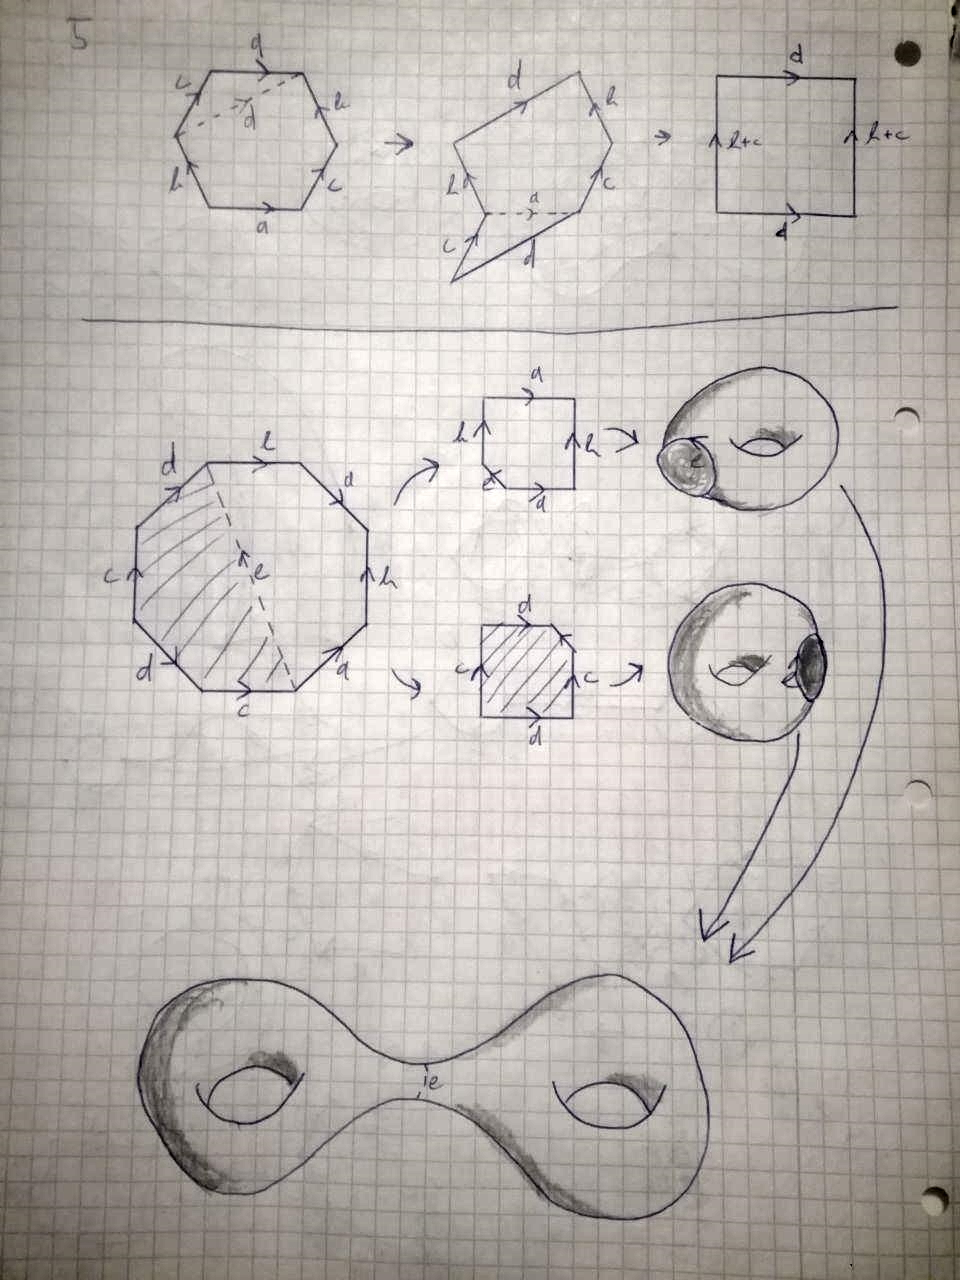
\includegraphics[width = \textwidth]{ue_img/9_5}
\end{figure}


\end{enumerate}


\end{document}


















